\begin{figure}[t]
    \centering
    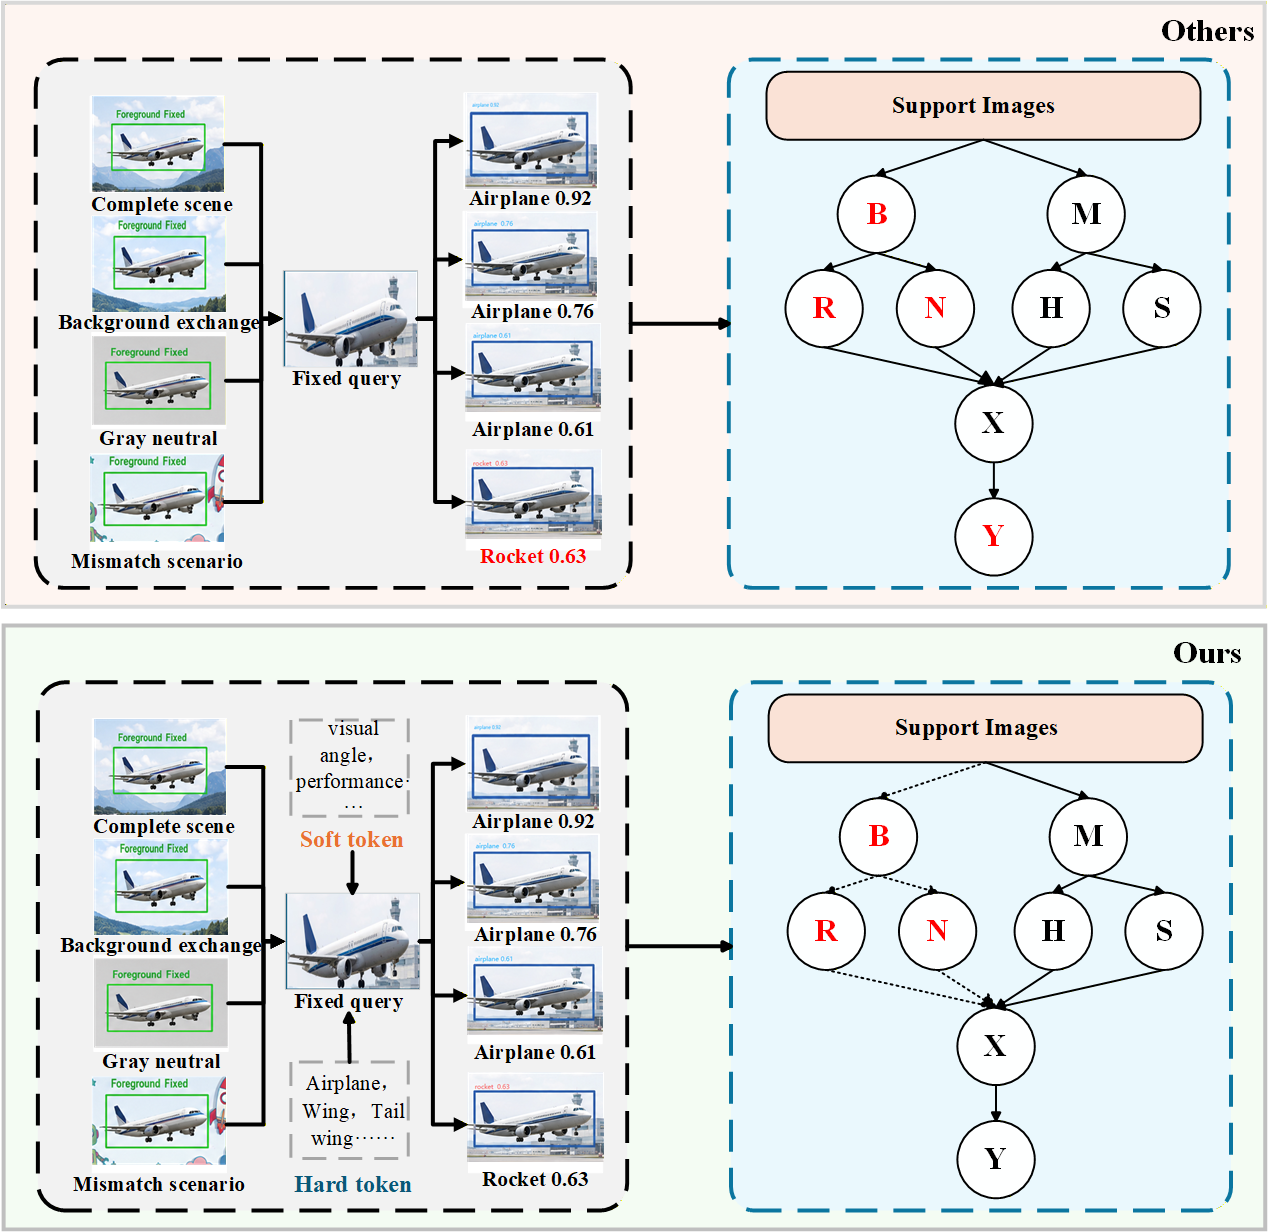
\includegraphics[width=\linewidth]{fig/context_leakage.png}
    \caption{\textbf{Motivation: support-induced context leakage.} \textbf{Top:} treating every support factor as valid evidence lets category-irrelevant context reach the query decision. With the support foreground, box, and query fixed, changing only the support context already shifts the confidence and, in the last row, the predicted category. \textbf{Bottom:} our framework separates category identity from domain appearance. A Hard token carries context-invariant identity, a Soft token carries only context-cleaned target appearance, and the authority routing decides how far either token may move the decision. Solid and dashed arrows denote retained and suppressed influences.}
    \label{fig:context-leakage}
\end{figure}
